\section{Exemplos}

\subsubsection*{Exemplo 1}


Uma linha que termina em uma reator e solicita a expressão no fim da linha, sendo esta suficientemente longa para desprezar reflexões. Assim, os dados e solução são apresentadas no código do MATLAB:

\lstinputlisting[language=Matlab,style=mystyle]{text/matlab/exemplo_1.m}

\begin{lstlisting}[language=Matlab,style=consolestyle]
>> V1_ref = 20;
>> V2_trans = 120;
\end{lstlisting}

Isso mostra uma tensão refletida de 20V e uma refratada de 120V. 

\subsubsection*{Exemplo 2}

Este exemplo fornece o modelo de uma linha com alimentação senoidal e com final como uma carga indutiva. Solicita-se a expressão para a tensão no fim da linha. Dito isso, uma vez identificado que o problema trata de uma linha com indutor, monta-se a função de transferência no domínio de Laplace do coeficiente de transmissão, com o intuito de facilitar os cálculos por meio das leis de Kirchhoff.

Na teoria a tensão senoidal da entrada também pode ser modelada no domínio de Laplace, multiplicada com o coeficiente de transmissão e logo em seguida ser aplicada a transformada inversa para obter a seguinte resposta no domínio do tempo: $v_f(t) = -0.901e^{-600t}+1.064cos(377t-32.14^{\circ})$. 

Esse resultado pode ser encontrado facilmente pela manipulação das equações transformadas. O interesse desse tópico é simular no MATLAB a resposta no domínio do tempo:

\lstinputlisting[language=Matlab,style=mystyle]{text/matlab/exemplo_2.m}

\begin{figure}[H]
\begin{center}
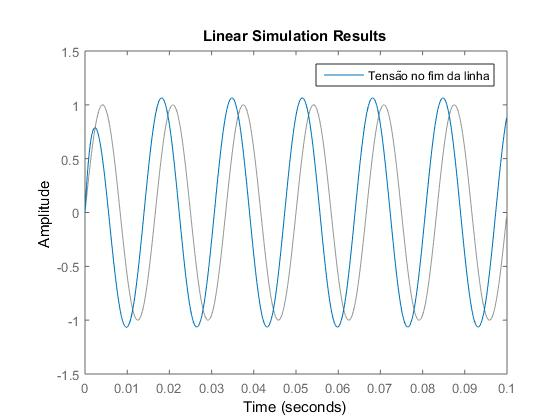
\includegraphics[width=12cm]{images/sim1.jpg}
\caption{Tensão no final de uma linha com reator na extremidade.}
\label{sim:1} 
\end{center}
\end{figure}

De acordo com a figura \ref{sim:1} observa-se um rápido transitório devido à presença da exponencial $e^{-600t}$ da resposta teórica. Como o argumento dessa exponencial é alto, seu decaimento é rápido e toma pouco mais de um ciclo para que seu efeito seja reduzido. O atraso de fase é presente devido aos $32.14^{\circ}$ de atraso na parcela cossenoidal.
\subsubsection*{Exemplo 3}

Este exemplo solicita a análise das constantes de tempo de ondas aplicada em uma LT com $Z=250\Omega$ e $f=60Hz$ ou $\omega = 277 rad/s$, energizada por um sistema cuja impedância equivalente é puramente indutiva. Potência de curto-circuito no valor nominal de tensão de $500kV$ de $25000MVA$ e $2500MVA$. 

Primeiramente identifica-se que o sistema é composto do tipo da seção "impedâncias internas de geradores" para o caso da indutância do gerador. Para esse caso a tensão que chega à linha é:


\begin{center}
    $v_1^{+}(t) = E_0(1-e^{-\frac{Z_1}{L}t})$
\end{center}

Portanto a constante de tempo será $\tau=\frac{L}{Z_1}$. Porém $X=V^2/S_{CC}$ e $L = X/\omega$, assim:

\begin{center}
    $\tau = \frac{V^2}{ \omega Z_1 S_{CC}}$
\end{center}

No MATLAB, para ambas as situações de potência de curto-circuito, tem-se:

\lstinputlisting[language=Matlab,style=mystyle]{text/matlab/exemplo_1.m}

\begin{lstlisting}[language=Matlab,style=consolestyle]
>> tau = [0.0013, 0.00013];
\end{lstlisting}

Isso implica dizer que um aumento de $10\times$ na potência de curto-circuito, ocasiona uma redução de $10\times$ na constante de tempo, com a redução do tempo implicando em um efeito menor da indutância.

\subsubsection*{Exemplo 4}

Este exemplo trata de uma  onda degrau que se propaga entre duas linhas com uma junção LC em série. Solicita-se a forma de onda da tensão no final da linha 2. Considerar as linhas com parâmetros idênticos e suficientemente longas para desprezar reflexões do ponto 2 em direção ao fim da linha. Novamente recorre-se ao auxílio do MATLAB para as operações algébricas para encontrar a equação transformada da tensão no final da linha:

\lstinputlisting[language=Matlab,style=mystyle]{text/matlab/exemplo_4.m}

A equação transformada para a tensão na linha 2 será:

\begin{lstlisting}[language=Matlab,style=consolestyle]
>> Vf =
>>            0.004167 s
>>  --------------------------------
>>  1.042e-06 s^3 + 0.002083 s^2 + s
>> Continuous-time transfer function.
\end{lstlisting}

\begin{figure}[H]
\begin{center}
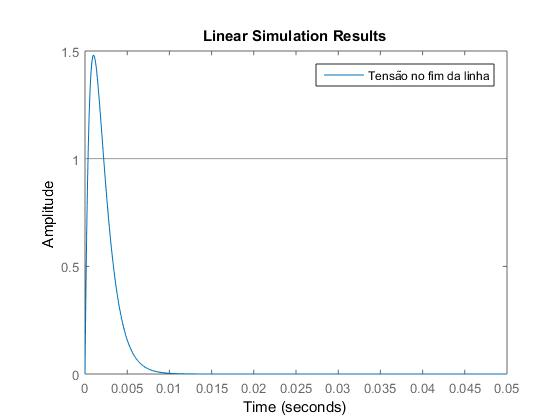
\includegraphics[width=12cm]{images/sim2.jpg}
\caption{Tensão no final de uma linha aberta com junção LC entre outra linha.}
\label{sim:2} 
\end{center}
\end{figure}

Transformando a representação no domínio de Laplace para o domínio do tempo, tem-se: $v_f(t) = 10.08(e^{-801.158t}-e^{1197.88t})$. Essa composição de exponenciais também pode ser confirmada na figura \ref{sim:2} referente à simulação.

Tanto pela equação teórica, quanto pelo gráfico da simulação, observa-se que para um tempo $t=0$, ambas as exponenciais valem a unidade e se anulam, resultando em 0. Em seguida para $t\longrightarrow \infty$ também resultado em um valor nulo, pois ambas as exponenciais também serão nulas.


\subsubsection*{Exemplo 5}

Neste exemplo solicita-se para determinar a tensão no terminal de uma LT protegida por um pára-raios quando atingido por um degrau de tensão de 1000kV. Impedância característica de $400 \Omega$. 

De acordo com a curva do problema, para uma corrente de até $1kA$, a tensão varia de $0kV$ a $300kV$; e no trecho da corrente de $1kA$ a $11kA$ a tensão varia de $300kV$ a $400kV$. 

Assim, dadas as equações linearizadas e não linear para a tensão no fim da linha:

\begin{center}
    $v_f = 2v_1^{+}-Z_1i$ \\ \vspace{1pt}
    $v_f=f(i)$
\end{center}

Para o caso linear, a solução será homogênea independente do trecho, de forma que: $v_f = 2000 - 400i$. 

Porém para o primeiro trecho em que a tensão cresce do zero a uma taxa constante $f(i) = 300i$, entretanto: $v_f = 2000 - 400i = f(i) = 300i$, implicando em: $i = \frac{2000}{300+400} = 2.85kA$. Esse valor de corrente viola o limite da trecho estabelecido de $1kA$. Para o segundo trecho a tensão varia com $f(i) = 10i + 290$ e igualando ao caso linear: $v_f = 2000 - 400i = f(i) = 10i+290$, logo $i = \frac{2000-290}{400+10} = 4.17kA$. 

Este último valor de corrente atende os requisitos do trecho e pode ser utilizado para modelar o circuito, de forma que a tensão $v_f$ pode ser calculada com a equação do caso linear, porém considerando $i =4.17kA$, resultando em $v_f = 33.17kV$.


\subsubsection*{Exemplo 6}

Calcular a tensão no terminal de linha para as condições de um raio que atinge a LT a uma certa distância do terminal de linha (proteção com pára-raios). A solução do problema beira a análise gráfico. Os dados fornecidos são uma corrente de surto máxima de $I = 10kA$, impedância característica da LT $Z_1=400\Omega$ e é fornecidas as curvas da forma de onda da corrente do raio e a curva VxI do pára-raios. Também considera-se:

\begin{equation} \label{exe:1}
\centering
\left \{
\begin{array}{cc}
i=0 \, se \, v_f \leq 1000kV \\
v_f = 10i+1000 \, se \, v_f > 1000kV\\
\end{array}
\right.
\end{equation}

Considerando simetria entre $v_1^{+}$ e $v_1^{-}$, tem-se: $v_1^{+}=\frac{Z_1i}{2}=200i$, apresentando assim a mesma forma da corrente, apenas escalonada. Assim, para o pico de corrente $10kA$, o pico de sobretensão é $2000kV$. A solução da saída pode ser obtida por: $v_f = 2(v_1^{+}-200i)$, isso causa um deslocamento vertical na curva em questão. 

\subsubsection*{Exemplo 7}

Este exemplo considera uma onda de tensão de $2000kV$ que atinge uma SE por uma impedância característica de $400 \Omega$ e se dirige a um nó com três ramos, dois deles resultam em LT com mesma impedância característica que a anterior e o outro ramo possui um pára-raios.

Como o pára raios é a carga não-linear, aplica-se o equivalente de Thèvenin do seu ponto de vista. Considera-se a mesma relação de tensão linear para o pára-raios que os problemas anteriores: $v_f = 1000-10i$. Tudo combinado resulta em uma tensão de $v_f = 1023kV$, segundo o código em MATLAB abaixo:

\lstinputlisting[language=Matlab,style=mystyle]{text/matlab/exemplo_7.m}

\newpage

